\documentclass{beamer}
\usepackage[utf8]{inputenc}
\usepackage[T1]{fontenc}
\usepackage[spanish]{babel}
\usepackage{amsmath, amssymb}
\usepackage{graphicx}

\usetheme{default}
\setbeamertemplate{navigation symbols}{}
\setbeamertemplate{footline}[frame number]
\definecolor{azultitulo}{RGB}{0,128,255}
\setbeamercolor{frametitle}{fg=azultitulo}
\setbeamerfont{frametitle}{series=\bfseries}
\setbeamercolor{title}{fg=azultitulo}
\setbeamerfont{title}{series=\bfseries}

% Si no se encuentra la imagen del histograma, se muestra un recuadro en su lugar
\newcommand{\histograma}[1]{%
  \IfFileExists{histograma_siniestros.png}%
    {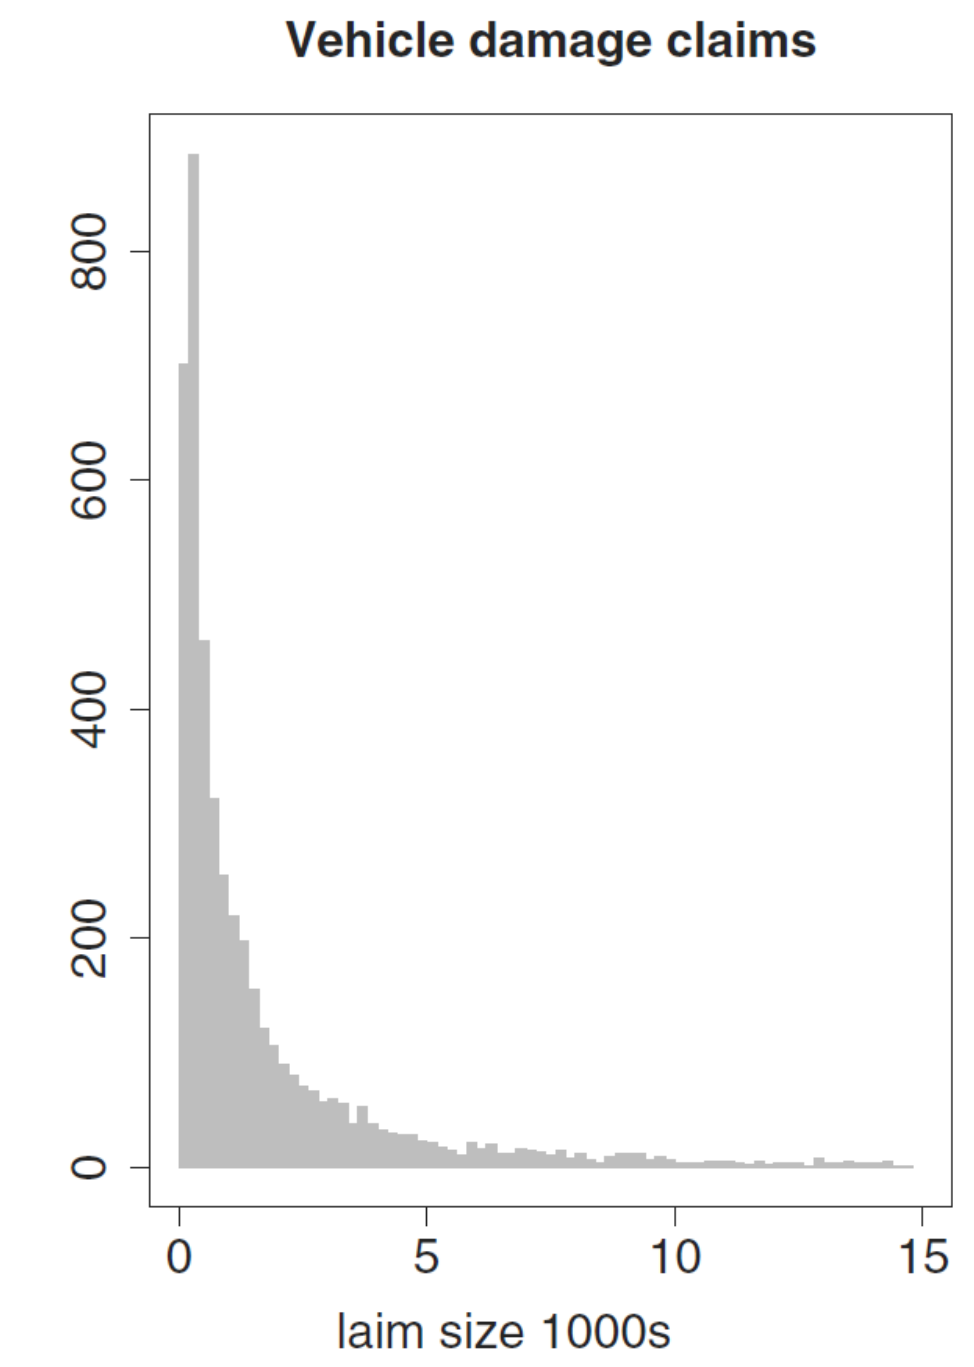
\includegraphics[#1]{histograma_siniestros.png}}%
    {\fbox{\parbox[c][4cm][c]{4cm}{\centering Histograma de\\ siniestros}}}%
}

\title{SME0823 Modelos Lineales Generalizados}
\author{Osvaldo Anacleto Jr}
\institute{ICMC-USP \\ \texttt{anacleto@icmc.usp.br}}
\date{2 de agosto de 2018}

\begin{document}

% ---------------- Página 1 ----------------
\begin{frame}
  \titlepage
\end{frame}

% ---------------- Página 2 ----------------
\begin{frame}{Estructura de la clase}
  \vfill
  \begin{itemize}
    \item Ejemplos de motivación
    \vspace{0.5cm}
    \item ¿Por qué estudiar Modelos Lineales Generalizados?
    \vspace{0.5cm}
    \item Estructura del curso
    \vspace{0.5cm}
    \item Familia Exponencial y MLGs
  \end{itemize}
  \vfill
\end{frame}

% ---------------- Página 3 ----------------
\begin{frame}{Ejemplo 1: siniestros de pólizas de vehículos}
  La figura de abajo presenta el valor (en miles) de $\approx 5000$
  siniestros ocurridos en una cartera de $\approx 68000$ pólizas de
  seguro de automóvil.

  \begin{center}
    \histograma{height=0.62\textheight}
  \end{center}
\end{frame}

% ---------------- Página 4 ----------------
\begin{frame}{Ejemplo 1: siniestros de pólizas de vehículos}
  Otras informaciones disponibles de las pólizas son:
  \begin{itemize}
    \item datos de registro del titular de la póliza: edad, género, dirección
    \item datos del vehículo: valor, antigüedad y tipo (autobús, furgoneta,
          sedán, convertible)
  \end{itemize}

  \vspace{0.2cm}
  \begin{columns}[T]
    \begin{column}{0.33\textwidth}
      \histograma{width=\textwidth}
    \end{column}
    \begin{column}{0.64\textwidth}
      \textbf{Posibles preguntas de interés:}
      \begin{itemize}
        \item ¿Es posible extraer información \textbf{relevante} de los
              datos disponibles de la cartera?
        \item ¿Cuáles son los factores que influyen en el valor del siniestro?
        \item ¿Es posible predecir el valor del siniestro para clientes
              potenciales?
        \item ¿Cómo determinar el \textbf{precio} de la póliza a partir de
              esta información?
      \end{itemize}
    \end{column}
  \end{columns}
\end{frame}

\end{document}
